In this project it was chosen to follow an iterative development process. This was chosen because the success criteria for this project are not well defined, since the goal of picking which song to play next is a largely subjective decision.

This project being very experimental, following a linear approach could require a large amount of research which has not previously been done, for making descriptive analysis and design documents, before being able to test our theses on how to cope with the problem. Problems which arise later in the process, would then not be handled in an efficient way.

One of the problem with the incremental model compared to the linear waterfall model is that the project can lack structure, since setting milestones with clear goals can be more difficult.


\subsection{Iterative Design Process}
In the iterative process, the design and implementation is done one step at a time. The development is done in iterations with a new milestone for each iteration. These milestones consist of some features which will be analysed, designed, implemented and evaluated, documenting every step in the process. Ideas for various algorithms will be tested on multiple subjects, which will be interviewed in an effort to find new possible problems or requirements, to be taken up for consideration in the following iterations.\kanote{ideer til algoritmer bliver testet på folk?}\\
We will be following these steps through each iteration:

\begin{enumerate}
  \item Gathering data from users and previous iterations
  \item An brief analysis of these data, for declaring new requirements
  \item A comprehensive design phase, researching and choosing concepts in solving these requirements
  \item An effective coding period, implementing the chosen design
  \item Evaluation, consisting mainly of black- and white box testing.
\end{enumerate}

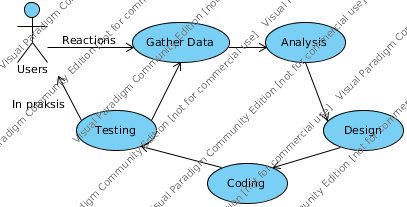
\includegraphics{Images/Developmentprocess.png}

\subsubsection{Iterations}
\textit{\textbf{1st iteration}}

	The project group set out with following milestones for the first iteration:

	Milestones:
	\begin{itemize}
		\item Initial data structure
		\item Be able to vote on a song
		\item Interview bars and pubs about requirements of a music system for their venue.
		\item Communicate a request for a song from one device to another and play it.
	\end{itemize}

	We started out with a requirement of being about to count votes on specific songs to, but we went a little behind schedule due unforeseen details about libspotify, so we simplified it to just communicating a one request.\\
	In conclusion this was too ambitious while not taking any obstacles in learning how to utilise the Spotify platform, in following iteration planning a margin for learning tools should be accounted for. Not every decision in the design phase was documented in the report, in addition not significant testing were made.

\noindent\textit{\textbf{2nd iteration}}

	On behalf of the experience made in previous iteration, about being to ambitious in meeting all milestones at deadline, another approach is introduced, by classifying each milestone under what "Must" and what "Should" be done this iteration. An emphasise will be put on documentation and testing on milestones of 2nd iteration:

	Must:
	\begin{itemize}
		\item Interview everyday users about requirements for music system.
		\item Do a section on concepts in the system
	\end{itemize}

	Should:
	\begin{itemize}
		\item Document previously taken decisions
		\item Describe architecture
		\item Do a comprehensive testing section
		\item Make a democratic handling on the backend
	\end{itemize}